\section{Introduction}
\label{sec:introduction}
\paragraph{}
\par The objective of this laboratory assignment is to study a circuit that contains two current sources, two voltage sources and seven resistors. The circuit has a dependent voltage source $V_c$ and an independent one $V_a$. One of the current sources is dependent, $I_b$, and an independent one, $I_d$. 
\par A representation of the circuit made with \textit{LibreOffice Draw} can be seen in figure \ref{circuit}.

\begin{figure}[H]
    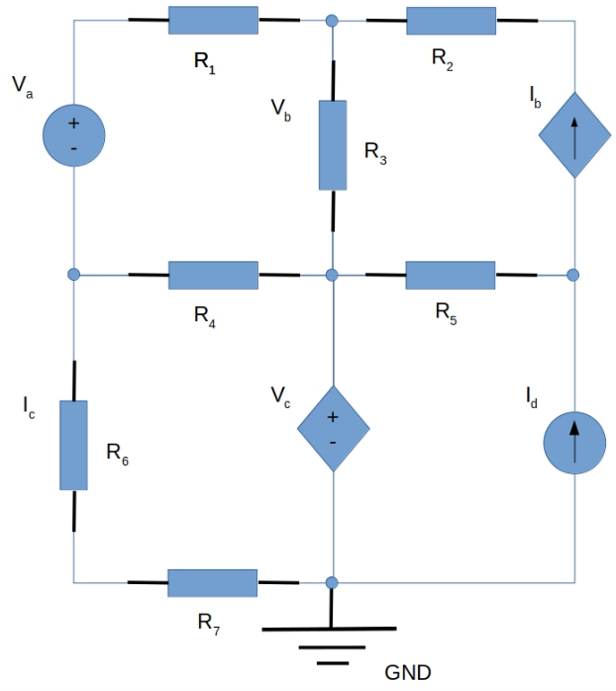
\includegraphics[width=0.4\linewidth]{Circuito.png}
    \centering
    \caption{Studied Circuit}
    \label{circuit}
\end{figure}

In Section~\ref{sec:analysis}, a theoretical analysis of the circuit is
presented. In Section~\ref{sec:simulation}, the circuit is analysed by
simulation, and the results are compared to the theoretical results obtained in
Section~\ref{sec:analysis}. The conclusions of this study are outlined in
Section~\ref{sec:conclusion}.

